%\documentclass[11pt,draft]{uvic}
%\documentclass[12pt,draft]{uvic}
%\documentclass[12pt]{uvic}
\documentclass[12pt]{uvic} 
%%% thesis.tex USING uvic.cls
%%%
%%% Options: draft => eps files shown as box with filename inside
%%%          10, 11, or 12pt => base font
%%%
%%% Michael Roth, 2001

%%% algorithm float
\usepackage{float}
\usepackage{subfloat}
\newfloat{algo}{ht}{loa}[section]
\floatname{algo}{Algorithm}
\usepackage{color}

%%% FOR SPACING (choose one)
\usepackage{setspace}
%\onehalfspacing
%\singlespacing
\doublespacing

%%% FONTS

\usepackage{type1cm}
\usepackage{courier}
\usepackage{mathrsfs}
\DeclareMathAlphabet{\mathpzc}{OT1}{pzc}{m}{it}

%%% FOR \citet and \citep

\usepackage{natbib}
%\usepackage{agu04}
\bibpunct{(}{)}{,}{a}{}{,} 

%%% FOR EXTENDED MATH

\usepackage{amsmath}
\usepackage{amssymb}

%%% FOR MODIFYING CHAPTER, SECTION STYLES

\usepackage{soul}
%\usepackage[nobottomtitles,compact]{titlesec}
%\usepackage[bf,small]{titlesec}
\usepackage[small,compact,raggedright]{titlesec}
%\usepackage{titlesec}

% \titleformat{\chapter}[display]
% {\normalfont\Large\bfseries}{{\thechapter}}{1em}{}
% \titlespacing*{\chapter}{0pt}{*1}{*2}
% %
% \titleformat{\section}
% {\normalfont\large\bfseries}{\thesection}{1em}{}
% %
% \titleformat{\paragraph}[runin]
% {\normalfont\normalsize\bfseries}{\theparagraph}{1em}{}
% %
% \titleformat{\subparagraph}[runin]
% {\normalfont\normalsize}{\thesubparagraph}{1em}{\ul}

% |\titleformat{\section}|\\
% |    {\LARGE\titlefont}|\\
% |    {\thesection}|\\
% |    {.66em}|\\
% |    {\ul}|\\
% \end{example}

%%% FOR MODIFYING CAPTION STYLES

\usepackage{array}
\usepackage{longtable}
\usepackage{multirow}
\usepackage[font=small,labelfont=bf]{caption}
% \renewcommand{\captionlabelfont}{\normalfont\bfseries}
% \renewcommand{\captionfont}{\normalfont}
% \setlength{\captionmargin}{12pt}

%%% USE URL FORMATTING PACKAGE
\usepackage{url}

%% Define a new 'leo' style for the package that will use a smaller font.
\makeatletter
\def\url@leostyle{%
  \@ifundefined{selectfont}{\def\UrlFont{\sf}}{\def\UrlFont{\small\ttfamily}}}
\makeatother
%% Now actually use the newly defined style.
\urlstyle{leostyle}

%%% YOUR OWN DEFINTIONS AND NEW COMMANDS (defs.sty)

\usepackage{defs}

%%% FOR LOADING IN TEXT FILES (APPENDICES)
%\usepackage{moreverb}

\usepackage{cancel}

%
% \makeatletter
% \def\input@path{{chapter1}{chapter2}}
% \makeatother
\makeatletter
\def\input@path{{data/}}
\graphicspath{{images/}}
\makeatother

%%% TITLE, AUTHOR, etc.

% \title{Fekete and Lebesgue Triangular Spectral Elements and Lagrangian
% Voronoi Diagrams}
\title{Optimizing Synchronization Cost for Mobile Devices using Expedient Trickle Sync}
\renewcommand{\titlestyle}{\large\bfseries}
\thesistype{Project}
\author{Brad J. BARCLAY}
\renewcommand{\authorstyle}{\large\bfseries}
\prevdegree{B.Sc., Brock University, 1999}
\degree{Master of Science}
\renewcommand{\degreestyle}{\large\bfseries}
\department{Computer Science Department}
\supervisor{Dr.\ Jens.\ WEBER}
\committeemember{Dr.\ Jens.\ WEBER, Supervisor %
(Computer Science Department)}
\committeemember{Dr.\ Bill.\ WADGE, Member % 
(Computer Science Department)}
\committeemember{Dr.\ Kui.\ WU, Member % 
(Computer Science Department)}
% \committeemember{Dr.\ M.\ Artian, Outside Member %
% (Department of Far Far Away)}
% in case you need two or more lines for that external, use tabular ...
%\committeemember{Dr. ?.\ ???????, External Examiner %
%(Institute of ?????????)}
% \committeemember{\begin{tabular}{c} 
% Dr.\ M. Foreman, External Examiner\\
% (Institute of Stuff Sciences, University of ???)
% \end{tabular}}
\copyrightyear{2008}
\copyrightpagedate{\today}

%%%

\pagestyle{plain}

%%%

%%%
\begin{document}

%%% Uncomment the following to see a graphic of the page layout
%\layout

%%% GENERATE TITLEPAGE

\pagenumbering{roman}
\maketitlepage
\makesupervisorycommittee

%%% ABSTRACT

%%% ABSTRACT
%%% optional argument in \begin{abstract}[...] gives style of title

\begin{abstract}[\normalfont\large\bfseries]
With the continued increase in the number of wirelessly connected mobile network devices, 
data synchronization for such devices has become an aspect of the lives of more and more 
users.  However, the synchronization process it still primarily stuck at the same technology 
level as in the mid 1990�s, utilizing a model that requires user-intervention to initiate synchronization.  This lack of intelligence can result in users basing decisions on potentially 
out-of-date information, and provides no mechanism for reducing the overall costs associated with network access during the synchronization process.  This paper proposes the development of a more advanced learning-based mechanism for synchronizing information 
for semi-connected mobile devices that attempts to synchronize data in the background, 
while minimizing both the tangible costs associated with network access in differing locales, and 
the less tangible(but often real) costs associated with presenting the user with out-of-date information. 
\end{abstract}


%%%

%%% GENERATE TABLES AND LISTS

\maketableofcontents
\makelistoftables
\makelistoffigures
%\makelistofalgorithms
%%%% LIST OF SYMBOLS / NOMENCLATURE

\chapter*{List of Symbols}
{\addcontentsline{toc}{chapter}{List of Symbols}}

\begin{center}
\begin{tabular}{*{2}{p{0.1\linewidth}p{0.40\linewidth}}}
\leb & Lebesgue constant & \lebmean & Chen-\babushka\ constant 
\tabularnewline
$\ell_i$ & Lagrangian/Cardinal functions 
\tabularnewline
$A$ & area 
\tabularnewline
$a_i$ & area/barycentric coordinates 
\tabularnewline
$\rho$ & density
\tabularnewline
$b_i$ & basis functions
\tabularnewline
$c_i$ & spectral coefficients
\tabularnewline
$L$ & Lebesgue function
\tabularnewline
$\{ x_i,y_i \}$ & set of nodes
\tabularnewline
$p$ & degree of polynomial
\tabularnewline
$n$ & number of nodes
\tabularnewline
$V_{ij}$ & Vandermonde matrix
\tabularnewline
$W_{ij}$ & integration weight matrix
\tabularnewline
$w_{i}$ & integration weight vector
\tabularnewline
$P_{n}^{(\alpha,\beta)}$ & Jacobi polynomial
\tabularnewline
$\mathscr{E}$ & electrostatic energy
\tabularnewline
$f$ & function
\tabularnewline
$f_i$ & $f(x_i,y_i)$
\end{tabular}
\end{center}


%%% ACKNOWLEDGEMENTS

%%% ACKNOWLEDGEMENTS
%%% optional argument in \begin{acknowledge}[...] gives style of title

%\chapter*{Acknowledgements}
\begin{acknowledge}[\normalfont\large\bfseries]

I wish to thank my supervisor for giving me just enough rope ...


\end{acknowledge}


%%% LOAD CHAPTER FILES

\afterpage{\pagenumbering{arabic}}
%%%\include{intro}
%%%
\chapter{Introduction}
%%%
\section{Introduction}

Mobile, semi-connected computing devices have quickly become one of the most dominant forms of personal data storage, data retrieval, and communications  devices on the planet.  Convergence has blurred the lines between what is a computation device, data storage/retrieval device, entertainment device, and communications device, to the point where many mobile devices have features of all four device types in them.  Mobile phones in particular can provide telephony, e-mail, instant messaging, music and video playback, games, imaging, and personal/business databases.  Such devices can run sophisticated software packages, and can often be used in the place of bulkier personal computer devices such as laptop computers.

Unfortunately, we still live in a world where network availability is not completely ubiquitous.  Cellular devices often have issues connecting to their network inside buildings, under overpasses, inside tunnels, and in sparsely populated locales.  For these reasons, applications written for mobile devices, particularly those which rely on some form of database, typically continue to require local storage to ensure data availability when network service is inaccessible.  Keeping this information up-to-date with respect to other databases requires data synchronization.

Of particular note, data synchronization for most mobile devices is still fairly primitive.  It may require the user to plug their mobile device in to a more traditional personal computer style device via a cable, and even when a wireless connection for synchronization is available, the user usually must initiate the synchronization process manually.  The device is typically unusable until the synchronization process has completed.  This may be acceptable for small databases which don�t change frequently (such as a personal address book), however for more complicated applications in business, government, and medicine, the requirements to be physically present with the device to be synchronized against (or potentially through), to manually enable and initialize the synchronization process, and to wait for the process to complete may be more onerous, and may work against the desire to ensure that the synchronized data is as up-to-date as is reasonably possible at the time the data is required.  For large data sets which change frequently, these requirements can become problematic, and can result in the user making decisions based on invalid data, and a reduced desire to use the tool for this purpose. Lengthy and onerous synchronization procedures may result in the user becoming lax in ensuring they synchronize frequently, increasing the chances that a cost may be incurred based on using invalid data.

Fortunately, mobile devices are becoming sufficiently powerful such that they can employ intelligence coupled with automated background synchronization to avoid these issues.  However, such intelligent synchronization systems have by and large not been put into place in favour of the status quo.  

Another recent innovation in many mobile devices is the ability to connect to multiple networks.  Mobile phones such as the Apple iPhone and Palm Treo are capable of connecting to cellular (GPRS, EDGE) and WiFi (802.11.a/b/g) networks for data transfer.  Each of these different network types typically have completely different data transfer rates and costs associated with them, with even identical networking technologies having different costs at different locales.  These differences can also affect the cost associated with data synchronization.

This project will propose an improved mechanism for synchronizing data with such devices, named Expedient Trickle Sync (ETS).  ETS is an intelligent, automated data synchronization system that synchronizes in the background, with the goal of reducing the overall cost of data synchronization in the following two areas:
\begin{enumerate}
\item By reducing the real cost associated with network access, and
\item By reducing the virtual cost associated with the users use of invalid or out-of-date data.
\end{enumerate}

\section{Research Scope}
The scope of this research is defined to be:
\begin{enumerate}
\item Identify and precisely specify the goals for the ETS algorithm,
\item Implement the ETS algorithm in a computer programming language,
\item Implement a simulation environment for evaluating the cost of a data synchronization algorithm,
\item Evaluate the ETS algorithm by running it through the simulator, along with both a purely random algorithm and a common, existing industry algorithm (HotSync).
\end{enumerate}

\section{Methodology}
Development of this project will be undertaken in three phases: the development of a synchronization algorithm simulation environment, the development and definition of the Expedient Trickle Sync algorithm, and the evaluation of the ETS algorithm within the simulation environment.

\subsection{Simulator}
Phase one will see the development of a simulator environment capable of running a given synchronization strategy algorithm across the course of many simulated days, calculating along the way the cost of synchronization using the strategy.  After a set number of simulated days, an average cost will be calculated and stored for the given sync algorithm.

The simulation will simulate a variety of elements, including the movement of the user from location to location during their simulated day (based on a definable schedule), the networks available in each location (and their associated cost , speed, and probability of signal loss), the users changing activity level in relation to the semi-connected mobile device, changes to the host database (which the mobile device synchronizes against), and user record access.  These latter two factors will be coded to occur based on Poisson processes \cite{RefWorks:32} (for determining when modifications or accesses are to occur), and a Normal distribution (for determining which records are affected by the modifications and accesses ascertained by the Poisson process).

\subsection{ETS Algorithm}
Phase two of the project is the definition of the ETS algorithm. This algorithm uses pattern analysis and intelligent heuristics to accomplish the following:
\begin{enumerate}
\item Make intelligent decisions as to when to initiate background synchronization sessions.  The decision as to when to synchronize is to be based on previous access patterns, with an attempt to minimize the real cost by synchronizing as much data as possible when in contact with low-cost, high-speed networks, and as little as possible when in contact with high-cost, low speed networks.  At the same time, it will attempt to minimize the virtual cost associated with using expired data by attempting to ensure that synchronization is frequent enough to maximize the probability that at time t, a record R required by the user is up-to-date, and
\item During each synchronization session, order the records to be synchronized so as to prioritize those records which have a high probability of being required between the time of the current synchronization ($t_{curr}$) and the next synchronization session ($t_{next}$), potentially synchronizing only a subset of the available modified records based on their predicted likelihood of being required during this time, if the network cost at $t_{curr}$ is significant.
\end{enumerate}

As the user is presumed to be mobile, the algorithm will need to deal gracefully with unexpected disconnection.  As the algorithm is a learning algorithm, it is expected to begin with no knowledge as to the users patterns or data needs, and will thus record these issues during the course of each day, improving its heuristics.

\subsection{Usage Model Study}
In order to obtain a real-world model 

\subsection{Evaluation}
The third and final phase will use the simulator to evaluate three algorithms against our simulated user:  the ETS algorithm, an algorithm analogous to the Palm HotSync �Slow Sync� protocol \cite{RefWorks:32, RefWorks:24, RefWorks:31}, an algorithm analogous to the Palm HotSync �Fast Sync� protocol \cite{RefWorks:32, RefWorks:24, RefWorks:31}, a random algorithm (which synchronizes random data at random times, used as a control), and simply not synchronizing at all (the "null synchronizer", also used as a control).  Each algorithm will be executed for a large number of simulated days, based on a model user, after which an average cost per day will be derived.  This average cost will be expressed as a simple polynomial, with a partial polynomial solution being provided through simplification using real-world cost profiles for data access on the various simulated network types.  These simplified polynomials will then be compared to evaluate how the ETS algorithm compares to the other two in terms of cost savings for both the real network access cost, and the virtual cost associated with using out-of-date or invalid data.  The simulation will be re-run across a series of model users, to evaluate how each algorithm performs under different usage scenarios.

The user models will be generated based on a real-world data, obtained from a proposed study of existing organizations which use existing synchronization solutions.  Details on the proposed study can be found in \ref{proposed_study}.

\subsection{Target Platform}
The language used for developing and deploying the simulator the simulator will be Objective-C v2.0 \cite{RefWorks:35} on Apple Inc. hardware.  While initially the simulation application will be developed to run a stand-alone single day simulation, if the simulation time is sufficiently large, the application may be modified to use an Xgrid controller \cite{RefWorks:36} to farm out simulated days to multiple systems running in parallel.

%%%
\chapter{Background} 
%%%

\section{Introduction}
People have long desired the ability to carry important information with them, as an aid to memory, as a portable resource, for entertainment, or to transport data from one location to another.  Throughout history, humanity has devised a variety of mechanisms for storing and transmitting data.

With the rise of the computer era, this desire for portable data access has continued; initially in the form of portable storage media such as the compact cassette and diskette, but more recently in the form of portable electronic devices which can act as both storage and access mechanisms, such as laptops, PDAs, cellular telephones, and portable media devices such as Apple�s iPod.  Initially, due to cost, size, and lack of infrastructure, these devices contained no wireless access capabilities, and thus required a wired connection to a network or desktop computer to be filled with existing digital information.  As this information changed over time on one device or another, the need to synchronize the two became imperative.

Even in the modern era, where wireless facilities are common in first-world countries, it is often still desirable to be able to physically carry data with us, as opposed to being able to access it over a network.  Cellular service may be sporadic at best inside buildings and vehicles.  WiFi connections only cover short distances, and thus lack coverage in all but a few locations.  Wireless network signals can be blocked, and downtime can be encountered.  Firewalls may block data access from certain locations, and certain locales may prevent access to certain types of data services by way of legislation.  As well, in under serviced areas, network contention and delay may be high, resulting in long wait times for desired data.  With the continued presence of these issues, in many problem domains it remains desirable to be able to maintain a local repository of data on the device, with synchronization services when a network connection is available to effect modifications to both local and remote data repositories.

Due to a lack of guaranteed connectivity, as well as a desire to be able to allow databases to be updated on two or more synchronized devices, these devices typically use optimistic replication \cite{RefWorks:6, RefWorks:22} for general synchronization services.  As we generally make no assumptions as to the types of data stored on such devices, pessimistic replication \cite{RefWorks:6, RefWorks:22} can be difficult to implement; if the set of records which might be updated on the mobile device is unknown at synchronization time, record-level locking becomes impossible when the device lacks a network connection.

For the purposes of this chapter we denote devices of this type to be semi-connected devices, wherein while they do provide some form of network connectivity, its presence at any given time $t$ is not guaranteed, and that $P_t$, the probability that at time $t$ the network is available, is not high.

The goal of this chapter is to describe the set of base requirements for optimistic replication when using semi-connected devices, based on the authors experiences surrounding his work developing the jSyncManager \cite{RefWorks:30, RefWorks:31}, a synchronization toolkit for PalmOS based devices, along with existing published research in relevant areas.  It will discuss synchronization topologies, mobile device connection and authentication issues, agreement on databases to be synchronized, selection of a specific database to synchronize, the mapping of records on both devices, the identification of modified records, identification of potentially conflicting records, conflict resolution, determining what information to include in an update packet, the writing of updated records and the removal of deleted records, updating synchronization metadata, and mobile device disconnection.

\section{Synchronization Topologies}
Two very important considerations for designing a synchronization system are determining how mobile devices and servers are to exchange data, and which systems in the synchronization network each device can connect to for a synchronization session. For the purposes of this paper, the set of all systems that can synchronize a specific database will comprise the synchronization cloud, and the devices in this cloud form a topology based on the rules of which other systems in the cloud they can synchronize against directly.

The topology of a synchronization cloud is akin to the standard network topologies.  Common such topologies, and how they are reflected in a synchronization cloud, include \cite{RefWorks:26}:
\begin{enumerate}
\item \textbf{Star}: (fig. \ref{sync-topologies}) in a typical star synchronization network, each mobile device connects solely to a centralized server.  Data modified on one mobile device propagates to any other mobile device through two synchronizations (mobile to server, server to mobile).  In this way, the synchronization strategy is one-to-one for the mobile devices, and one-to-many for the centralized server device.
\item \textbf{Ring}: (fig. \ref{sync-topologies}) in a ring synchronization network, each mobile device and/or server in the cloud synchronizes with two other devices in the cloud.  The devices in the cloud chain together in this way, with the last device in the chain synchronizing against the penultimate device in the chain and the first device in the chain.  While the synchronization rules can be relatively simplified (as each device only synchronizes against two known, fixed devices), it may take up to $n/2$ synchronization sessions for a piece of data to propagate through the network.  In addition, adding new devices to the network can be highly disruptive, requiring a portion of the chain to be broken, and the new device inserted.  The data synchronization in this sort of network is easily broken if one mobile device in the system is not synchronized for a lengthy period of time, and devices adjacent to each other in the ring require that their users are frequently in close proximity to each other to permit the synchronization.  For these reasons, ring topologies are generally unknown in practical use.  Ring topologies require a one-to-many synchronization strategy for all devices in the cloud.
\item \textbf{Tree}: (fig. \ref{sync-topologies}) in a tree synchronization network, each mobile device synchronizes with  single, fixed device (typically a server).  These servers, in turn, may synchronize against  higher-level server, eventually leading to a single root server.  In the tree model, the mobile devices are the leaves of the tree, with the servers making up the root and inner nodes.  Leaves synchronize using a one-to-one strategy, inner nodes and the root node synchronize downwards (towards the leaves) in a one-to-many strategy.  Inner nodes synchronize upwards in a one-to-one strategy.  This model is best when the synchronization cloud is geographically distributed;  various subsets of the mobile devices synchronize against their own local servers, and these local servers synchronize against high-level servers, and eventually with the root server, which disseminates modifications downwards throughout the cloud.  In a worst-case scenario, the dissemination of data between any two mobile devices in the cloud will be the length of the root paths between the two most distant leaves in the tree.  However, in usage scenarios where the locality of data is important, the number of synchronizations required for local data updates between two mobile devices will typically be two.
\item \textbf{Complete}: (fig. \ref{sync-topologies}) in a complete synchronization network, any member of the synchronization cloud is permitted to synchronize directly against any other member of the cloud.  Thus each device employs a one-to-many model of synchronization.  In a best-case scenario, a modification made to a given mobile device can be effected to any other mobile device in a single synchronization.  However, in practice it may take a significant amount of time for a change to propagate its way through the entire cloud, and if a subset of devices only ever synchronize amongst themselves, changes made within that subset may never propagate to other devices in the synchronization cloud. One solution to to this problem is to ensure that all servers synchronize against all other servers on a regular basis, and that all mobile devices in the cloud synchronize with at least one server on a regular basis.
\item \textbf{Hybrid}: (fig. \ref{sync-topologies}) several hybrid approaches may be taken.  One common hybrid approach has all of the mobile devices acting as nodes in a star network, which is centred with either a ring network or complete network of servers.  In this way, the mobile devices synchronize against one (or more) servers, and the servers synchronize against each-other.  In such hybrid models, the mobile devices may be permitted to synchronize with any server, or may be fixed against which server they may synchronize with.
\end{enumerate}

\begin{figure}[htb]
\centering
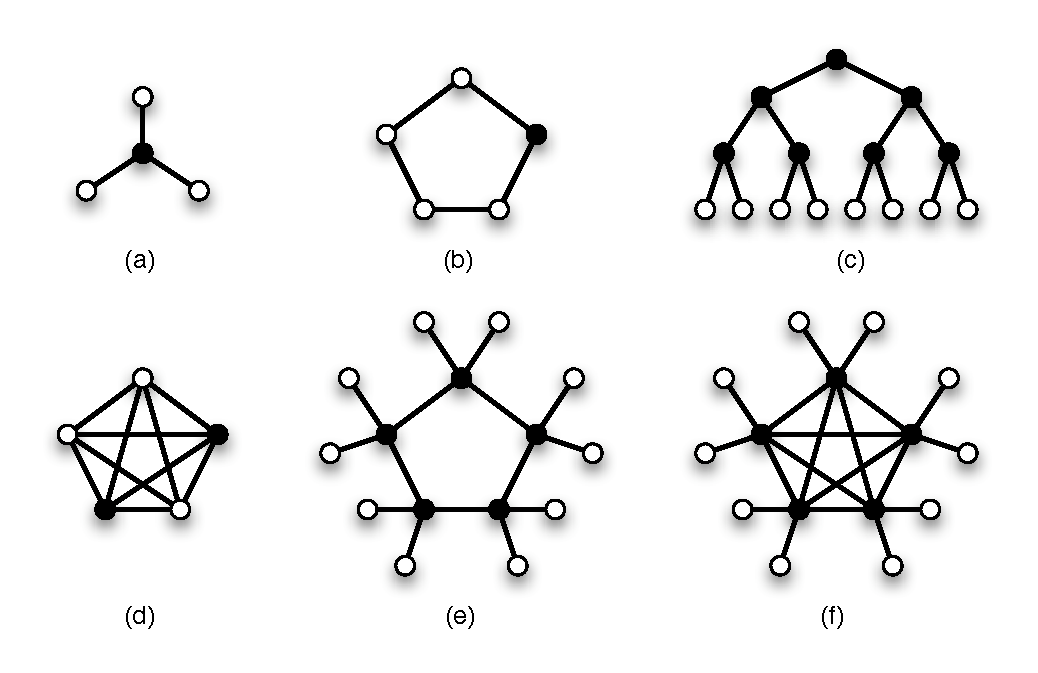
\includegraphics[width=\textwidth]{Figures/topologies}
\caption[Synchronization Network Topologies]{Synchronization Network Topologies.  White nodes denote mobile devices, black nodes denote servers.  (a) Star. (b) Ring. (c) Tree. (d) Complete. (e) Hybrid Star/Ring. (f) Hybrid Star/Complete}\label{sync-topologies}
\end{figure}

\section{Connection and Authentication}
The first requirement to be identified is the ability to connect the mobile device to the synchronization host.  How the connection is made can vary greatly between different classes of devices, with varying protocols and connection methods employed.  Mobile phones may use Bluetooth or USB connectivity to a host, or may use a TCP socket encapsulated within a General Packet Radio Service (GPRS) or Enhanced Data rates for GSM Evolution (EDGE) wireless connection.  WiFi through 801.11b/g is also an option on some portable phones.  Handheld devices, such as those from Palm Inc., may connect using Bluetooth, USB, RS-232 serial, infrared, modem, or WiFi connectivity using a custom protocol stack (HotSync), either directly or encapsulated within TCP packets.

Once a network connection of any type has been made, it is typically important to authenticate the device against the host in some manner, to ensure that the device and its owner are permitted access to the system in question.  Oftentimes in situations where devices are connected in a physical manner proximal to the synchronization host, this step may either be skipped, or simply used to verify whether or not the given device has synchronized with this system previously.  Devices that synchronize through proximity wireless systems such as Bluetooth may simply rely on a pre-existing Bluetooth pairing of the host and the semi-connected device for the purposes of authentication.  WiFi enabled devices may also contain no explicit authentication, requiring the user to configure as appropriate either WEP or WPA style WiFi authentication.

Such simple authentication mechanisms are common on most semi-connected device types, outside certain specialized device types \cite{RefWorks:12}.  Common commercial handhelds and mobile telephones lack any form of authentication outside authenticating against the network itself.  Perhaps more important is host or database level access authentication.  An important consideration in designing an authentication mechanism is the fact that semi-connected devices are portable by their nature, typically relatively valuable, and are both targets for theft and loss.  Under such circumstances, it is desirable to prevent an unauthorized user of the device from being able to either access the existing data on the device, or to be able to connect to the synchronization host to retrieve more data (or to potentially corrupt data within the hosts database by purposefully synchronizing in bad information).  While access to the existing data on the device needs to occur outside the scope of the data synchronization process (and is thus outside the scope of this paper), access control to the synchronization host thus requires the ability to both authenticate the device, and to authenticate the user of the device.  In situations that require high levels of data security, authenticating both becomes important as it both prevents unknown users from accessing or modifying data on the synchronization host, and as it prevents authorized users from substituting their own devices.

Device and user authentication may take several forms.  Device authentication may be performed via hardware identifiers (e.g. CPU or system serial codes), via cryptographic certificates, or a combination of the two.  User authentication is typically best performed using an external factor authentication, such as a password, biometric validation, or through proximity to a personal security device carried by the user.

Once authenticated, various levels of data access may be granted or barred based on the credentials of the device and the user.  Access may be granted only to specific databases, or it may affect which records inside a given database are acceptable for transfer.  As well, once authenticated, handshaking may occur to enable data encryption for all further synchronization requests and responses during the session, so as to keep data inaccessible to man-in-the-middle attacks.

Other forms of handshaking and global data synchronization may also occur as part of the connection phase, such as device capabilities an characteristics, which may affect how synchronization is to proceed.  Very basic data synchronization tasks such as time synchronization, which do not necessarily belong to any specific database or type but which are of global use, may also occur as part of the connection phase.

\section{Agreement on Databases to Synchronize}
Once the connection has been initiated and authenticated, an agreement needs to be arrived upon to determine what databases between the semi-connected device and the synchronization host need to be synchronized.  Part of this agreement may involve connecting the mobile device to a remote database, routed through the synchronization host, and any associated authentication required between the synchronization host and the remote database, the mobile device and the remote database, or both.
Selection of the databases to synchronize is dependent upon the application support on the handheld, the databases available on (or to) the synchronization host, any authorization rules and permissions in place, and the ability of the mobile device and/or the synchronization host to synchronize the data types exposed by those databases.  Only when all of these criteria are met can a database be synchronized between the device and the host.  Thus, the selection of the databases to be synchronized is the subset of all databases available on the device and on the host that fit the above requirements.

There are a variety of ways in which the device and the host can determine which elements fit into this subset.  This may be achieved through a handshaking phase where the two devices agree upon the subset of databases to synchronize, or it may be driven primarily by one of the systems involved.  The later situation is common for PDA-style devices, where plug-in units called conduits \cite{RefWorks:12, RefWorks:31} are run in sequence at synchronization time, each testing the mobile device to see if the data they wish to synchronize is available.  If it is not available, the conduit can either exit gracefully (permitting the next conduit in sequence to run), or construct and initialize a new database to use for synchronization purposes \cite{RefWorks:31}.

Note that while this scenario has the advantage of the mobile device not needing to have the database to be synchronized at connection time, it has the disadvantage of requiring that the necessary conduit be installed at connection time on the host computer.  As such, while the presence of a conduit on the host system can permit synchronization where the portable database is missing, the presence of the database on the mobile device alone is insufficient to permit synchronization.

\section{Selection of a Database to Synchronize}
Once the subset of databases to be synchronized has been agreed upon, one of these databases may be selected for synchronization.  There are a variety of mechanisms for selecting which database should be synchronized next at any given time.  The simplest mechanism is to simply iterate through the list of databases in whatever order they occur in the subset of databases to be synchronized.  Using this mechanism doesn�t require any computation, and thus selection is fast:  at the beginning of synchronization, select the first database in the set, and iterate through the list thereafter.  This system may encounter problems in situations where a single application has multiple database to be synchronized, as there may be a necessary order for the databases to be synchronized.  For example, it may be necessary to ensure that a common encryption key database be properly synchronized before the databases which rely on this key are synchronized.

A refinement to this approach is to use an application-centric view of synchronization, where an entire application consisting of multiple databases is synchronized as a single unit.  In this situation, while the order of the applications is not guaranteed, the order of the databases synchronized as part of that application can be guaranteed.  This model is easily exposed when using host-side conduits for synchronization control, as each conduit can manage the databases it needs in whatever order it desires, however there is no guarantee as to what order each conduit is giving the opportunity to exchange data.

This latter model can impose efficiency penalties under certain circumstances.  In the case of a database which is shared amongst multiple applications, each conduit accessing the database may either force it to be synchronized multiple times needlessly, or at the very least needs to check to see if the data has been synchronized by a previous conduit and skipped.

An enhancement that gets rid of the need to check whether a database has already been synchronized during an existing session is to implement the notion of priority to the database selection.  Using this system, the database synchronization order can be determined by ordering the databases by a stored priority value, synchronizing the database with the highest priority first, and the database with the lowest priority last.  Under such a system, any shared databases that require synchronization prior to applications which rely on them can be given a higher priority, and thus are guaranteed to be synchronized earlier in the process.

The use of a priority field comes with its own set of difficulties.  Firstly, the handling of databases that have the same priority cannot be done in any guaranteed order;  it is usually a documented limitation of such systems that there is no guarantee of ordering between databases with the same priority.  Secondly, it is possible for application developers to abuse the priority ordering by simply marking themselves as the highest priority level.  This can be mitigated by allowing an administrator control of the priority levels for each database, using the application-defined priority as a default value.

\section{Mapping of Records on Both Devices}
Once a database has been selected for synchronization, it is up to the synchronization system to determine (or provide) a mechanism for mapping the records from both the host and the mobile device.  As each system may store this information in differing formats, it can be very difficult to know that record x on the mobile device mates up with record y on the synchronization host.  This is complicated by the assumption that the data may differ between the two devices (thus necessitating the synchronization process).  It is further complicated by the fact that the host and the mobile device may use different identification values for the same record.  However, even with these challenges present, it is a requirement to be able to match a record between the mobile device and the synchronization host in order to determine whether it requires synchronization, which fields need to be synchronized, and to ensure that the correct record(s) are updated on both devices.

The mechanism used for determining the record mapping can affect the time taken to perform the synchronization task.  Linear scanning of the records from one system containing n records against the other system containing m records, using a suitable matching algorithm between the two systems would require on average nm/2 comparisons.  This could be lengthy for very large databases, and may easily exceed the users patience in such situations.

The simplest solution to the mapping problem is to ensure that both the mobile device and the synchronization host use the same identification numbering system for records.  An unsigned 32-bit value is usually sufficient for mobile device synchronization, as it permits over 4.2 billion unique record IDs.  Dividing this address space in half can ensure that new records created on both the mobile device and the synchronization host between synchronization sessions do not overlap.

However, it is often the situation that either one or both sides of the synchronization solution are developed by different groups or even organizations:  while one may be in control of the host-side database, they may be synchronizing against a vendor-supplied mobile database that uses a differing identification system.  Or one may find oneself in the situation of wanting to bring mobile device synchronization into an organization which has entrenched host-side applications from third-party vendors, for which you do not have control of the database.  Additionally, the mobile device�s operating system may impose its own record identification scheme (cf: PalmOS).

In situations where control over the unique identifiers on one or both devices exists, maintaining identical identifiers on both ends of the process may be difficult or impossible.  In such a situation, another mapping mechanism needs to be developed.  One such mechanism is to maintain a mapping database for conversion between one identification scheme and the other.  Depending on the synchronization needs, this can be implemented as a hash, with one side�s identification scheme serving as the key, and the remote end�s mapping serving as the value associated with each key.  Maintaining a second hash for the reverse direction may also be desirable in a variety of situations.  Keeping two such hashes in proper synchronization with each other becomes an important added task, as does persistent storage of such a map, for use during subsequent synchronization sessions.

Finally, in situations where one has no control over either the host systems or the mobile systems record identification mechanism it may be impossible to maintain a unique record identifier (often because one or both sides uses a third-party application which doesn�t maintain a unique identifier for each data record).  In such situations, one of the records fields may need to serve as a unique identifier, with a matching heuristic used to find the matching record (if any) on the other devices database.  Such a situation is typically less desirable, as scanning all the records to build the mapping at synchronization time may require significant runtime.  This process can also be problematic in situations where multiple records share the same unique identifier field (such as two calendar appointments for the same date and time), or where the unique identifier field for a record on one of the devices is modified (such as the name of a contact in an address book).  In such situations, the mapping heuristic may need to take other record field data into account to attempt to find the mapping, however if a record on one end of the synchronization is sufficiently modified, finding this mapping at synchronization time may become impossible for the system to do in an automated way.

\section{Identification of Modified Records}
Assuming a mapping of records between the mobile device and the host database selected for synchronization is possible, it is important for us to be able to identify specifically those records on both devices which have been modified since the last synchronization session.  For the purposes of this paper, we define a modified record to be one which falls into one of the following categories:
\begin{itemize}
\item\textbf{Added}:  Records that have been newly added to one of the databases since the last synchronization session between the two devices;
\item\textbf{Updated}: Records that existed at the time of the last synchronization, but which have one or more fields which have been modified in either database since the last synchronization session;
\item\textbf{Deleted}:  Records that have been removed from one of the databases since the last synchronization session.
\end{itemize}

Identification of the modified records is an important facility, as in an attempt to minimize the synchronization time and minimize the amount of data that needs to be transferred, we need to separate the records that have been changed since the last synchronization session with the given host from those which have remained identical \cite{RefWorks:15, RefWorks:17}.  Records which have not changed between synchronization sessions on one or both devices do not need to be synchronized, and thus require no records to be updated on either device.

Modified record identification can be most simply implemented using a single per-record flag that is set whenever a record has been modified.  If these flags are cleared after every synchronization session, any records so flagged will have been modified since the last synchronization.

An alternate system is to always record a modification date/time for each record, as well as the date/time for each synchronization.  Using this system, we can select only those records with a modification date since the last synchronization date.  Note that while this system is relatively easy to implement and process, the task of ensuring that multiple host clocks are synchronized together with the mobile devices can make implementing such a system for multiple-host synchronization scenarios difficult.

Identifying records using either of these methods does introduce some issues, however.  In particular, once a modified record has been identified using this scheme, it is necessary to identify which of the three types of modifications has taken place (added, updated, deleted).  Added records are easy to identify if we have a good mapping system in place to match records between the device and host; added records will be those which exist on one device, but which have no mapping to any records on the other device.  It is worth noting that in the case where mapping occurs via field comparison heuristics, added records may be mistaken for existing records if the identification fields correspond sufficiently closely.  That is, if record A2 (record 2 on device A), a newly added record, is heuristically matched to record B1 (which normally maps to record A1), the later update phase will run its update routine on B1, modifying it to an incorrect state.  Later in the synchronization (or in a subsequent synchronization session), the system may determine that B1 and A1 now differ, propagating the bad record data back to the original device as a different record.  For this reason, if heuristic record mapping is to be used, a sufficiently intelligent heuristic must be developed to prevent mismatches.

Identification of deleted records can be complicated if the record on the system where it has been deleted is erased (that is, where no record of it having existed on the system and its status as having been deleted has been recorded).  In this case, a deleted record on device A may in fact be mistaken as a new record on device B, thus causing deleted records to re-appear after every synchronization session.  As such, a mechanism for detecting deleted records is necessary.

Identifying deleted records can take several forms.  In one algorithm, we do not erase between synchronization sessions, but instead flag them as having been deleted.  In this case, it is important for applications using the database to simply ignore deleted records.  At synchronization time, deleted records on each device can be identified, with the deletions synchronized between hosts.  To conserve space on mobile devices when using this algorithm, it may be desirable to remove the data for the record, maintaining  just the records metadata until synchronization time.  Deleted records may be truly erased once the synchronization session for the database is complete, as part of the post-synchronization cleanup (for two-way synchronization), or may continue to be flagged for deletion and erased once all hosts have flagged the record as deleted (for n-way synchronization).

In another algorithm, we make use of a record identification map to find records that are in the map, but which do not exist in the target database;  if they are in the map, they existed in the database during the last synchronization session, and if they no longer exist, they must have been deleted in the intervening time between the last synchronization and the current synchronization.  The record can then be deleted from the other device.  This deletion can generally be total erasure.  Once the deletion is complete, the mapping information for this record between these two systems can be removed (although other mappings for the deleted record may exist between a given device and other hosts for multi-way synchronization scenarios).

In scenarios without any deletion metadata, identifying deleted records may require a complex heuristic.  Lacking any reliable metadata on which to base a decision, however, it may not be possible to correctly identify whether a record has been deleted on one system, or is simply missing on that system and should be copied from the other.  This situation should be avoided whenever possible, as it can result in unreliable results.

Any record that has been identified as having been modified, but which hasn�t been added or deleted, must by elimination be treated as updated.  Updated records can be detected by comparing mapped records between the two devices and detecting differences.  There are a wide variety of algorithms that can be used to compute a hash for a record on both devices; this hash can then be compared, and if different (assuming we use the same hashing criteria) can be marked as having been updated since the last synchronization.  If one end of the synchronization maintains a modified record or a modification date and last synchronization date, we can determine which record (if not both) was updated since the last synchronization.  Note however that if neither side maintains such information, determining which side contains the updated data will again be difficult: with a modified field that exists on both databases we will be unable to determine which version is the updated record and which was the original.  Likewise, with a field that exists on one device but not the other, it becomes impossible to determine whether that field was added to one device (and thus requires update to the other), or if the other device has this field removed (in which case it should likewise be removed from the first device).  Note that using a mechanism where we compare record hash values (or where we simply compare fields directly) is generally unsatisfactory in terms of synchronization time and the amount of data that needs to be transferred, as each set of records must be read and compared.

Once we are able to identify individual modified records, a sub-problem can be to communicate the set of modified records to the other end of the synchronization session in the fewest possible packets of data.  In the situation where one (or both) devices are unable to determine for themselves which records have been modified since the last synchronization (i.e.: when the records of both devices need to be compared to determine if modifications have been made), such an optimization is difficult, and has generally not been undertaken.  This sort of synchronization is often denoted as slow sync in the relevant literature \cite{RefWorks:1, RefWorks:2, RefWorks:24, RefWorks:31}.

In the situation where both sides are capable of identifying which records have been modified independently, however, we can apply various protocols for communicating precisely which records have been modified since the last synchronization session.  One algorithm (typically denoted as fast sync in the relevant literature \cite{RefWorks:2, RefWorks:22, RefWorks:31}) involves a request-response style protocol, where one end of the synchronization (the requester) sends a request for the next modified record in the relevant database.  The responder responds either with the next modified record in an iteration of modified records, or a code denoting that no further modified records are available.  This protocol thus requires only $n + 1$ packets (where n is the number of modified records in the database) to request all of the modified records in iteration in a one-way synchronization.

An interesting alternative method that has been proposed is Characteristic Polynomial Interpolation (CPI) \cite{RefWorks:2, RefWorks:24}.  In this scheme, characteristic polynomials are derived on both devices using their set of available records IDs.  We treat these sets as being part of a sufficiently large finite field, so as to constrain  the size of the polynomial evaluations, and to ensure integer evaluations for divisions.   Once the polynomials are derived, both devices use a set of agreed upon sample points to evaluate their characteristic polynomial.  These evaluations are then sent to one of the hosts, which then interpolates these values by solving a generalized Vandermonde system of equations  The zeroes of the resulting polynomials are determined, which results in the set differences for both devices respectively.

CPI Sync has the significant benefit (as presented) of not requiring a system of modified flags nor modification date/time to determine which records on both hosts are new since the last synchronization.  However, as the zero solutions to the interpolated function only give us those records that exist on one host but not the other, it is only ideal for the case where we want to detect new records that exist on one device, but not the other.  While not presented in \cite{RefWorks:24}, given a mechanism for independently determining which records have been modified, we can run a second round of CPI Sync using the modified records on both devices as the subset.  The resulting zero solutions of the interpolated function are thus the records that have been modified on one device, but not the other (as an interesting side effect, if we compare the solution values against the set of local records known to be modified, those local records which have been modified but which do not appear as a solution can instantly be flagged as having been modified on both devices, and hence potentially in conflict).

While \cite{RefWorks:24} maintains that CPI Sync is thus often requires significantly fewer packets than slow sync, and discusses how fast sync functions (and further compares fast sync performance to slow sync performance), it fails to compare the performance and number of packets required for synchronization to fast sync.  While this data is not discussed nor present in \cite{RefWorks:24}, we can derive some expectations.  If we assume that we perform two rounds of CPI Sync to determine both the added and modified records (as proposed above), for n modified records we would need to transmit at least $n + 2$ packets for a one-way synchronization (one for each round of evaluations in CPI Sync, plus one to request each modified record).  Without the second round of CPI Sync to determine the modified records, the entire algorithm boils down to that of slow sync.  As such, it appears that CPI Sync is best suited for applications where data is only ever added, and not modified, and even in this case it does not appear to ever perform better than the fast sync protocol.

\section{Identification of Conflicting Records}
Another important challenge occurs when we find that two records that map to each-other on both the mobile device and the synchronization host have both been modified since the last synchronization session.  When this occurs, the records are said to be in conflict.  For the purposes of this paper, we identify the following conflict types between two systems device A and device B:
\begin{enumerate}
\item Two records with identical identification information was added to both A and B since the last synchronization,
\item A record was modified on either A or B, and was deleted on the other device since the last synchronization.
\item A record added to either device A or B, and was independently added and later deleted from the other device since the last synchronization,
\item A record was modified on both A and B since the last synchronization.
\end{enumerate}

Note that the situation where a record was independently deleted from both A and B since the last synchronization is not  typically considered a conflict, as deletion typically entails the same act on every database (i.e.: the record is simply no longer required).  In essence, in such a situation the data is already synchronized for us purely by circumstance, and the situation can be safely ignored (with any required final erasure of the records on both sides being performed as necessary).

Conflicts are often the most difficult situations to be resolved in data synchronization, and nearly always entail the use of a heuristic to resolve the conflict \cite{RefWorks:18, RefWorks:22, RefWorks:27}.  When this heuristic is imperfect, it may cause a situation where the merged data differs between the two devices after the synchronization session is complete, thus either forcing these records to be synchronized again during the next synchronization session, or appearing to the user as a failure in the synchronization process (as both devices now contain different data for the same record).  Minimizing errors in the merge process is thus key to user satisfaction in synchronization systems.

Complicating matters, user activity can cause merge conflicts that are difficult to detect and manage.  For example, if a user accidentally deletes a record and decides to restore it manually (by re-entering the record information by hand), it is possible that they may modify (either purposefully or inadvertently) the data being entered in such a way that its mapping with other synchronized databases is lost (e.g.: in a system that identifies records by a computed field hash, if one of the hashed fields is misspelled, uses different type case, etc., resulting in a new hash).  In such a case, where the user expects the system to realize that the re-created record is supposed to be the same information as was stored in the accidentally deleted record, the system might in such a case decide that it is a new record, and handle it as such.

Detecting these conflicts is thus of high importance in the synchronization process.  The system for determining the set of conflicting records typically depends upon a comparison of the modified record metadata available on both devices.  In the case where modified since last synchronization flags are in use, detecting a conflict simply requires finding the subset of all records where a given record has its modification flag set on both the mobile device and the host system.  In a system that uses a modification time and last synchronized date field, conflicting records are those which have been modified on both the mobile device and host system since the last synchronization time.

For systems which do not employ synchronization metadata, detecting conflicting records requires the comparison between all pairs of mapped records.  In such a case, however, it is often difficult to determine whether a given pair of mapped records which exhibit differences are simply modified on one side and unmodified since the last synchronization on the other, or whether a conflict exists.  For this reason, the merging algorithms on such systems are often complicated and error-prone \cite{RefWorks:27}.

It is worth noting that two identical records may appear to be in conflict.  This typically occurs when the user inadvertently thwarts the synchronization process by manually modifying a mapper record pair on both the mobile and host system with identical data.  In such  situation, modification flags and/or times may indicate that a record is in conflict, however an examination of the data on both may show that they already contain the same record data.  In such a situation, no action needs to be taken other than to update the synchronization metadata for the records.

\section{Conflict Resolution}
Once the set of all pairs of conflicting records has been determined (if any), the conflicts must be merged together to create a record which contains the details of both modifications.  Merging is typically the most computationally intensive operation of a data synchronization system, and a variety of merging strategies exist \cite{RefWorks:6, RefWorks:22, RefWorks:27}.

It must be noted that the merge strategy in use for a synchronization system is typically dependant on the data involved.  Different data types will have different merge strategies depending on the type of conflict, and the way the data is to be recorded on the device.

In some situations, the data may be presented as a listing where a merge simply involves appending any new data to the end of the old data.  This is particularly common for text-based data.  Merging such information can be done in a similar fashion as with version control repository synchronization tools such as the Concurrent Versioning System (CVS) or Subversion.  Note that in the case of the source code synchronization tools, merge conflicts can still occur at the line level, repair of which requires user attention \cite{RefWorks:6, RefWorks:8}.

For complex records that contain a number of short, simple fields however, handling merge conflicts can be more troublesome.  The simplest algorithm to deal with such conflicts is to permit the user to specify a global preference as to which side of the synchronization should take precedence in the event of a conflict.  With such a setting available, when a conflict occurs the higher-precedence devices record field data overwrites the lower-precedence devices matching record field.  It is also possible to simply ask the user on a record-by-record basis \cite{RefWorks:33}, however this is often undesirable in situations where the synchronization is to occur without user intervention, as is typically the case where large data-sets are involved.

In systems where fields have a modification time stamp, it is possible for the merge heuristic to simply choose the field with the latest time as being appropriate.  While this assumption of appropriateness is not guaranteed to be correct, it is suitable for use when it is significantly more important for future synchronization sessions that the data is consistent, as inconsistencies can lead to a variety of cascading synchronization problems.

Next, assuming the applications to be synchronized are designed with it in mind, it may be possible to retain both sets of field data within one field, so that the user can choose which version of the field is correct after synchronization (typically the next time the record involved is accessed).  Any modification to the field (i.e.: the user deleting the invalid version of the field data) will cause the record to be synchronized during the next session, at which time the record will be repaired on the next synchronized device.

Finally, in certain cases it may be possible to average differing numerical values to come up with a new value that is between the two claimed values.  While this sort of synchronization is of much more limited use, it is implemented in Cristian's clock synchronization algorithm \cite{RefWorks:37}. 

\section{Determining what information to include in the update packet}
In order to affect changes to a remote record once the differences have been determined and any conflicts have been resolved, the modified data needs to be sent across the communications line to the remote device.  Typically when synchronizing semi-connected devices, the more capable system (typically the synchronization host) takes care of these more computationally intensive operations (due to its greater available RAM, faster processing speed, and larger secondary storage facilities).  Once the system has determined the updates to be made on the remote device, it has to construct an update packet containing the new record information.

As we typically wish to minimize the time required to synchronize the devices, it is highly desirable to minimize the data to be transmitted.  This is particularly so for semi-connected devices, as their network connectivity may at times incur a monetary cost from the amount of data transferred, the time taken to transfer the data, or both \cite{RefWorks:13, RefWorks:25}.  As such, minimizing the size of the update packets (along with minimizing the number of update packets) is highly desirable.

There are a variety of mechanisms for reducing the amount of data required for an update packet.  One relatively obvious method is to simply use a lossless compression algorithm on the record data prior to transmitting it as the update packet to the remote device.  This method should be able to achieve an improvement in the update packet size, however it does incur a time penalty for compression and decompression.  This is of particular importance on the mobile device, which typically has significantly less computational power than a desktop or server machine.  For databases containing thousands of records, the added computation required to generate or process an update packet may become noticeable to the end user on slow, low-power, or memory constrained devices.  Hardware compression and decompression in the network transport link layer can mitigate this disadvantage, however mobile devices often omit such hardware due to space and cost constraints.

A second option is to prune down the data contained within the update packet.  While many synchronization systems effectively merge the entire record on the host or server side, and transmit the new record data to the mobile device as a whole, it is possible to construct a synchronization system that provides only the modified and merged fields, along with a set of field identifiers \cite{RefWorks:5}.  The field identifiers are used to denote the specific fields being changed by the update packet, along with those changes.  In this way, small changes to records with a significantly large number of fields can be transmitted in a potentially significantly quicker manner \cite{RefWorks:5}.

Further refinements may be found by expressing field modifications not as their absolute final state, but by the difference between the old state and the final, synchronized state \cite{RefWorks:8, RefWorks:34}.  The suitability of a field-level difference calculation to a synchronization solution may depend strongly upon how radically field are changed.  If changes are typically relatively small, then transmitting only the differences may make sense, however in cases where data that is modified does typically change radically, such a system may in fact increase the amount of data that needs to be transmitted when used in conjunction with the elimination of unchanged fields from the update packet \cite{RefWorks:34}.  In cases where the typical change level is difficult (or impossible) to quantify, a flag could be used to differentiate between fields that have been expressed as a difference from their previous value, and a field which is presented as a wholesale change.

Ultimately, if the processing power of the handheld device doesn�t present a significant issue, and if the data (and the type of typical modifications) permit it, a combination of all three mechanisms may prove best, whereby field modifications are expressed as differences (or not, depending on the level of field change), only those fields which have been modified are transmitted (along with field identifiers so the receiving device can effect the same changes or replace the field as appropriate), and this update packet compressed using a suitable lossless compression algorithm to minimize the data that needs to be transmitted, thus minimizing the time required to complete the synchronization process.

One special case is the update packet for deleting a record on the remote device.  Such an update packet typically only requires the unique record identifier used by the remote device, along with a flag or command to denote that a deletion of the record needs to take place.  Newly added record update packets, while treated the same as those for other types of update packets, may require that the remote device return the unique record identifier for the newly created record, if the transmitter and received do not use the same record identification scheme.  In this case, the returned unique identifier is used to update the record mapping information for future synchronization sessions.

\section{Writing Updated Records and Removing Deleted Records}
Upon completion of generating the update packet(s), they must be transmitted to the remote device, which decodes them, determines the type of modification to take place, and affects the necessary modification to its own target database.  The specific steps to be taken are dependant upon the design of and information contained within the update packet itself, along with the structure of the database on the device being updated.  The data presented in the update packet may require modification or conversions to fit within the target database.  All of this is highly dependant upon the database design and target application, and thus cannot be suitably covered here.

One special consideration to note is the disposition of deleted records towards the end of the synchronization session.  For cases where deleted records maintain a record of their existence (so as to determine which records have been deleted at synchronization time), once the deletion has been synchronized with all expected synchronizing devices it may be permanently erased from the system \cite{RefWorks:22}.  This is typically most significant for the mobile device, which typically has less available data storage facilities than the host(s) or server(s) it synchronizes with.  

Determining when to remove these deleted record stubs is important, particularly in a multi-node synchronization solution.  In the case where each mobile device synchronizes with only one synchronization host (one-to-one synchronization), removal of the stubs on the mobile device can be achieved immediately after each synchronization session.  However, in situations where the mobile device must synchronize against multiple hosts (one-to-many synchronization model), these deletion stubs may need to be retained.  In the situation where a mobile device synchronizes against a fixed number of other devices in the synchronization cloud, these stubs should be retained until they have been synchronized against each of the assigned devices.  

In situations where the number of devices the mobile device synchronizes against is highly variable (such as in a complete synchronization network), these stubs need to be maintained until they have propagated to every other node in the network.  As a given mobile device may not synchronize against every other member of the synchronization cloud directly, and as those devices may have synchronized with other devices which have been synchronized against the mobile containing the original deletion stub prior to synchronizing against that mobile device itself, we cannot easily determine when the deletion has propagated to all devices in the cloud.  As such, a heuristic may be required to prevent these stubs from consuming mobile device memory unnecessarily; in the simplest form, these stubs may only be retained for either a fixed amount of time \cite{RefWorks:22}, or for a fixed number of synchronizations (or for some hybrid of these two values), trusting that devices in the cloud it has not synchronized with directly will eventually get the deletion information through other devices it has synchronized with.  Another possible heuristic is to keep the deletion stub until it has synchronized with at least one server device; again, the strategy takes advantage of the assumption that the server will eventually propagate the deletion to all other devices in the cloud.

Likewise, any stored record mappings to or from any given deleted records ID can likewise be expunged from the system, once they are no longer valid.  Doing so helps keep such mapping data to a size linear to the total number of synchronized records in the database, keeping the search time against such mapping tables relatively stable over time.

\section{Updating Synchronization Metadata and Disconnection}
To ensure the coherence of future synchronization sessions, any synchronization metadata must be updated.  For synchronization systems utilizing modified flags, the flags associated with the cloud member being synchronized against must be reset, such that all records show as being unmodified (when compared to the current cloud member being synchronized against) since the last synchronization.  This permits us to properly determine those records which have been modified since the current synchronization \cite{RefWorks:2, RefWorks:31}.

For synchronization systems utilizing a last synchronized time stamp,  the time at which the synchronization of each record was completed needs to be updated \cite{RefWorks:6, RefWorks:22}.  As well, the last synchronization time needs to be recorded.  Choosing the time for last synchronization time is important, particularly in scenarios where there are more than two devices in the synchronization cloud.  Setting the last synchronization time too late (such as at the end of the synchronization session) can cause data loss in future synchronization sessions; records modified on another mobile device between the beginning of the synchronization and the time when the last synchronization time is recorded may be missed on subsequent synchronizations (as they will appear to be mode prior to the last synchronization time), however recording the last synchronization time at the beginning of the synchronization session may cause issues if the synchronization fails to complete.  For this reason, the best policy it to record the beginning of the synchronization session for a given database as the last synchronization time, but to only commit this information if the synchronization completes correctly.

At this point, assuming no further databases require synchronization between the two devices, they may disconnect.  The disconnection may be initiated by one side of the synchronization session by sending a disconnect message to the other device, or one device may simply disconnect at the protocol layer, terminating the connection.

It must be noted here that as mobile devices are semi-connected, an inadvertent disconnection could occur at any time.  Wireless connectivity could be easily lost by moving outside of the range of the wireless access point, or by moving into a dead spot (caused by a wall, overpass, building, etc.).  Batteries could also fail during the synchronization process, forcing a shutdown of the mobile device.  For this reason, it is important to be able to distinguish between intentional and unintentional disconnections, and to have suitable strategies for when an unintentional disconnection does occur, to ensure correct behaviour during the next synchronization session.

\section{Conclusion}
Data synchronization is a complex process, with many significant points of breakage.  A variety of synchronization algorithms are possible, some with greater potential for breakage and data loss than others, but where limitations may be in place due to a lack of control of the design of one of the databases involved.  Designing a synchronization system is complicated, requiring a careful analysis of the type of data being synchronized, how the mobile devices are expected to connect to the data within the synchronization cloud, and how the data is to flow through all the devices in the synchronization cloud network in a timely manner.  Security, authentication, and data access rights cannot be ignored in most complicated synchronization environments, and for certain data types, legal restrictions and requirements may necessitate a very thorough analysis of the data-flow, to ensure that security and confidentiality are strictly adhered to.

The lack of a dedicated connection to any sort of network, and the ability for that connection to be lost at any time is the paramount consideration when designing a synchronization solution.  As these devices are designed to be mobile, synchronization services must expect that at any point in time during the synchronization process that the user could leave the wireless coverage area, and yet still desire to use the device and the data it contains.  For this reason, a synchronization solution for a mobile device must be graceful in its handling of lost connections.  Dealing with such unknowns is a significant challenge for designers of mobile device synchronization solutions.

Regardless of these issues, in a world where mobile devices have increasing capacities and capabilities, but where available wireless connectivity cannot be simply taken for granted, the need for better synchronization solutions will only continue to increase, and thus further research and development continues to be warranted.

%\begin{figure}[!ht]
%\centering
%\ifpdf
%\includegraphics[width=1.0\textwidth]{}
%\else
%\includegraphics[width=1.0\textwidth]{Figure.eps}
%\fi
%\\[5mm]
%\caption[This line appears in the table of contents] {This is my caption ...}
%\label{Fig:725}
%\end{figure}


%%%
\chapter{Simulation Environment}
%%%

\section{Introduction}

The purpose of the simulation environment is to provide a consistent mechanism for evaluating the cost and efficiency of various synchronization protocols.  It takes a series of configuration parameters as input which describe the characteristics of the environment we wish to simulate along with how long to run the simulation, and outputs a linear equation expressing the average cost per day for the synchronization algorithm in question.

In this chapter, we'll explore the environmental elements being simulated, the mathematical models used to drive the simulation, how the simulation logic is controlled, the protocol used to communicate with synchronization adaptors, along with a discussion of the functionality of the three synchronization protocols developed to compare the ETS protocols effectiveness against.

The simulation itself runs at a resolution of one-second intervals.  We define a \emph{tick} to be a simulated one second interval within the simulation.

\section{Simulated Elements}

The goal of the simulation environment is to evaluate the overall cost of a synchronization algorithm by following a model user through a series of days as they synchronize their wireless mobile device through a programmed series of locations.  Within each location there may be a variety of network types available, each with their own cost structure and data transfer rates.  These elements will each be presented in this section.

\subsection{Networks}

As we are evaluating the synchronization costs related to wireless mobile devices, we require some form of network transport for the transmission of synchronization data and metadata within our simulation environment.  These are expressed as a series of network objects, one per network which our sample user may intersect during the simulated day.

The networks each have three primary attributes inside the simulation:  their transfer rate expressed as bytes per second ($N_{rate}$), the cost associated with each byte transferred ($N_{cost}$), and the probability per second that the connection can be lost ($P_{connection lost}$).  Each of these elements is an important part of the simulation execution, as they permit the simulation to determine the duration of a series of network operations, their related monetary cost, and at which probability a connection may be lost during a synchronization session.

\subsection{Locations}

A location is a specific geo-physical region that the user may be within during their simulated day.  A location is simply defined by zero or more networks which are accessible within that location.  Note that a given network may exist within multiple locations; for example, it is expected that generally a cellular network will be available in most locations within most urban areas.  Thus, the relationship between locations and networks is an N:M relationship.

\subsection{Locales}

Locales build upon the physical locations by layering atop them temporal information; thus a locale is a location along with a time in which that location is entered.  This is used to permit the simulation to change from one location to the next during the duration of the simulated day.

Along with the time in which a location is entered ($L_{entry}$), the locale also provides information on both the frequency of synchronization ($L_{sync frequency}$), and the number of expected mobile database accesses ($L_{expected accesses}$).  These are described internally as the expected number of synchronizations per second, and the expected number of accesses per second.  Note that we typically do not expect a user to make multiple synchronization requests nor to have multiple database accesses within a a single second; as such these values are expected to be represented by small positive fractions.

Through the use of locale objects, we can permit the user to enter the same physical location at different times of day, with different mobile device usage patterns.  For example, a user who telecommutes from home and who uses their mobile device frequently during the normal work day may have a high expected database accesses value during business hours, but would have an exceedingly low expected database accesses at night while asleep.  In such a case the location is static, but the users usage patterns change.  Thus, the relationship between locations and locales is 1:N.  As the days are simulated from time 00:00:00 until time 23:59:59, the first defined locale is automatically entered at 00:00:00, and the last defined local persists until 23:59:59.

\subsection{Records}

A record is the smallest unit of data exchanged during the synchronization process, and represents a logical unit of compound information.  For the purposes of the simulation, we do not actually model the record or its data, but instead simply maintain a record identification number, size, and revision number.  The identification number ($R_{ID}$) is used as a matching mechanism between a record stored in the mobile database and a record stored within the server database.  The size ($R_{size}$) is used for calculating how long it will take to transfer the record, as well as how much its transfer will cost.  Finally, the revision number ($R_{revision}$) is used as a mechanism for comparing matching records within the mobile and server databases to determine differences between the records.

The revision number is of particular importance, as it is used in two different contexts within the simulation environment.  Firstly, it is used during a mobile database access by the simulated user to assess whether to increment the intangible cost factor which relates to the use of out-of-date information; if the revision number of the mobile database record $M_k$ is less than that of the matching record on the server database $S_k$, the intangible cost factor is incremented by the difference $S_k - M_k$.  Secondly, it is used to provide the synchronization protocol implementation with a list of records requiring synchronization, returning the set of all records with identification number $k$ where $S_k > M_k$.

While it is possible for the record size to be specified manually, the record size is typically assigned during the simulations set-up stage randomly based on a Normal distribution (\ref{gaussian}).  In this way the records can be generated with varying sizes, with a pre-set mean and variance.

Records also have an implicit probability of access by the user of the mobile device.  The simulation assumes that records are not evenly used, but that instead certain records are accessed more frequently than others.  This is intended to model typical real-world experience with databases.  While this probability is not stored within the record itself, it is based on a records ID number and the total number of records within the database containing it.  This will be discussed further in sub-section \ref{databases}.

\subsection{Databases}\label{databases}

A database is a logical collection of records.  For the sake of the simulation environment, databases are always of a fixed size.  The system maintains two separate simulated databases, one for the server, and one for the mobile device.  Ideally, for the intangible cost of synchronization to be zero, these two databases should be identical at all times.  However, in the typical situation, it is expected that these two databases will in fact differ for the bulk of the simulation run.

The server database $S$ maintains an expected number of modification arrivals per second and a maximum number of simultaneous modification arrivals.  Using a Poisson Process (\ref{poisson}), a series of probabilities are calculated between $0$ and $S_{max arrivals}$ inclusive, using the expected number of modifications.  During every simulated second, a random value is selected and compared against this series of probabilities to determine how many records should be modified during the current simulation time.  Once a number $v$ between $0$ and $S_{max arrivals}$ has been selected based on the calculated probabilities, $v$ records within the database are selected for modification.  These $v$ records are selected at random using a Normal distribution (\ref{gaussian}), such that the record with ID $S_{max}/2$ has the highest probability of selection, and the records with ID $0$ and $S_{max}$ have a very low probability of selection, with all other values having a probability falling upon a Normal curve.  Once each record to be modified has been identified, its revision number $R_{revision}$ is incremented by one.

The mobile database $M$ handles whether or not the user has viewed a record during each one second interval in the simulation, based upon the expected mobile database accesses value stored in the current locale object.  During every tick, we choose a random number $n$ and compare it to the expected mobile database access rate per second in $L_{expected accesses}$.  If $L_{expected accesses} >= n$, an access has occurred.  We then determine which record has been accessed during this interval in a manner identical to that of how we determine which record to modify in the server database $S$, using a Normal distribution.  In this way the most-modfied records on the server are also the most frequently accessed records on the mobile database.  Unlike the server database, however, mobile database accesses are limited to one per tick, and as such form a Bernoulli Process (\ref{bernoulli}).

\subsection{User}

Tying the above simulated elements together is the user object ($U$).  Only a single simulated user exists within a simulation run, and they persist throughout every simulated day.  The user object maintains the list of locales available to the user, and manages the transition between one locale and another during the simulated day.  As such, the user object maintains a 1:N relationship with the locale objects.  The user object also contains the single instance of the mobile database, and as such has a 1:1 relationship with the mobile database object.

\section{Models}

Manipulation of the simulated elements is governed by a series of mathematical models, which dictate the behaviour of the simulation process by ensuring the simulated elements remain within realistic bounds.  The models transform pseudo-random numbers into values within a defined range in order to simulate unknown information that falls within a known (or expected) set of bounds \cite{RefWorks:38, RefWorks:40}.  This section details these models as they are utilized within the simulation environment, along with the rationale for their selection.

\subsection{Pseudo-Random Number Generation}\label{random_nums}

A key ingredient to simulating discrete, random events is the reliable generation of random numeric values \cite{RefWorks:38}.  For simulation, it is generally desirable to generate values which are as close to uniformly distributed within the interval $(0, 1)$ as possible.  As it is impossible to generate random values using purely deterministic techniques \cite{RefWorks:38}, we must choose a pseudo-random number generator (PRNG) algorithm which produces uniformly distributed numeric values, with an extremely long period between repetitions.  Additionally, the pseudo-random number generation algorithm should produce random values very quickly, as an algorithm which requires a large number of instructions may cause our simulation to require significant runtime to arrive at a result, as a single simulation run may require tens of millions random numbers (indeed, based on experimentation a one year simulation can easily require in excess of 30 million random values).  Thus, a balance between the appearance of randomness, long period, equidistribution, and computational efficiency is the ideal trait of a pseudo-random number generator for use in our simulator \cite{wiki:mersennetwister}.

The PRNG selected for the simulation is the Mersenne Twister algorithm /ref{mersennetwister}, as it meets all of these requirements.  It's period before values start to repeat themselves has been proven to be $2^{19937}-1$, has a very high order of equidistribution, passes numerous statistical tests for randomness, and is fast.  In testing during PRNG evaluation for the simulator, the LGPL Mersenne Twist implementation used \cite{mersennetwistcode} was slightly more efficient than the Mac OS X built-in random number generators \texttt{rand} and \texttt{drand48}.  The fact that the efficiency is not worse than the platforms random number generator, coupled with its improved equidistribution and significantly longer period make it an excellent choice for discrete event simulation \cite{mersennetwister}.

\subsection{Normal Distribution}\label{gaussian}

Characterizing the types of data that can be synchronized in a generalized manner is nearly impossible;  the types of information that are can be synchronized are as varied as any other form of computer data.  In addition, without studying a specific and widely adopted synchronized database, it is nearly impossible to generalize the access frequency of the records within the database.





\subsection{Bernoulli Process}\label{bernoulli}


\subsection{Poisson Process}\label{poisson}



\section{Controllers}

Talk about the control elements of the simulation (time controller, sync controller, sync logic controller, etc.)

\subsection{Time}
\subsection{Cost Controller}
\subsection{Synchronization Controller}

\section{Synchronization Adaptor Protocol}

Talk about the way we define a synchronization protocol here.

\section{Comparative Protocols}

\subsection{Null Synchronizer}

Talk about the null synchronizer here

\subsection{Random Synchronizer}

Talk about the random synchronizer here.

\subsection{Slow Synchronizer}

Talk about the "slow sync" synchronizer here, and discuss how it models the mechanism used by HotSync, ActiveSync, iSync, etc.

\subsection{Fast Synchronizer}

Talk about the "fast sync" synchronizer here, and discuss how it models the mechanism used by HotSync, ActiveSync, iSync, etc.

\section{Conclusion}

Conclude this chapter on the synchronization environment.

%%%
\chapter{Expedient Trickle Sync Algorithm} 
%%%

\section{Introduction}  

The sole goal of the Expedient Trickle Sync (ETS) algorithm is to reduce the cost involved with data synchronization.  It does so by considering two factors:  the cost involved with physically transferring bits across a network, and the cost conceptually incurred when the user makes use of out-of-date data.  These two factors are frequently diametrically opposed:  the network cost can easily be reduced to zero by never synchronizing any information, however the cost involved with the use of out-of-date data increases exponentially.  Conversely, we can synchronize at a high rate of frequency to minimize the probability of using out-of-date information, however this can be at the expense of using more network time and resources than is otherwise necessary.  Thus, minimizing the cost of synchronization is a fine balance between ensuring the data the user is most likely to need is up-to-date, while minimizing the frequency and amount of time spent synchronizing.

The ETS algorithm attempts to minimize the cost of synchronization via four heuristic sub-algorithms:  determining when to synchronize, determining which available network to synchronize with, determining which subset of records to synchronize, and lastly by prioritizing the synchronization order.  While the intent of these four sub-algorithms is to reduce the overall cost of synchronization, they are not designed to guarantee absolute minimal synchronization cost; additionally, as they are based in part on a statistical analysis of the users past needs, sudden changes in a users habits could potentially circumvent these algorithms.  However, as these new user patterns take hold, the algorithm can learn from them in order to once again attempt to minimize the network cost; as such, the goal in cost reduction of the ETS protocol may not always be optimal when measured across short durations, it should approach an optimal level over the long term.
  
\section{Determining when to synchronize}

Determining when the synchronize so as to minimize cost is an extremely complex task.  At a one-second resolution, there are $2^{86400}$ possible sets of synchronization points.  Determining which members of these sets have the minimal cost in a rigourous manner would be inordinately computationally intensive, and thus is completely infeasible.  As such, a heuristic mechanism which will quickly reduce the cost of synchronization with minimal computation is desirable.  Such a heuristic must be suitable for running on a mobile device, and thus cannot require significant computing power or memory.

To fulfill these requirements, an algorithm which we can very quickly evaluate is important.  Easily calculated and recorded values, such as those pertaining to the probability the user will need a record on the device within a specified interval of time, how long it has been since the device was last synchronized, and the cost of synchronizing on the least expensive network in the mobile devices current location are excellent candidates for creating such an algorithm.

The mechanism selected for the ETS algorithm to use is to combine the above mentioned values into an equation, such that high probabilities and time since last synchronization have an increasing influence on the expression, and where high cost has a decreasing influence on the expression.  The derived value is then compared against a threshold value ($T$):  if the value is greater than the threshold at the time it is computed, we initiate a synchronization session, otherwise we do not.

In specific, given the probability function $P(x)$ which generates the probability that the user will access a record on the mobile device during the fixed-size interval of the day $x$, $\Delta t$ is the time since the last synchronization session, and $C_{byte_{net}}$ is the cost of transferring one byte of data on the selected network, then we define the function $G$ as:
\begin{equation}
G(x) = \frac{(\frac{8}{15}*P(x+1)+\frac{4}{15}*P(x+2)+\frac{2}{15}*P(x+3)+\frac{1}{15}*P(x+4)) * \Delta t}{C_{byte_{net}}}
\end{equation}\label{threshold_function}
Note that in the function $G$ we evaluate the mobile device record access probabilities of the next four time intervals, with each subsequent interval having half the influence of its immediately preceding interval.  In the default implementation, the intervals are 15 minutes in length; thus the probability calculation takes into consideration the next hours worth of usage.

Calculation of these probabilities is based upon a table maintained by the ETS algorithm, which stores the number of record accesses for each time interval in the day, for each of the last seven days.  In order to keep computation simple, the quantity of records accessed within each interval is not considered, only whether or not \emph{any} record was accessed during the interval; the probability algorithm is interested only in the probability of a record being accessed each day during the specified interval, and not how many were accessed during each interval.  Thus, an interval $x_a$ which has accesses in the seven preceding days of $\{1, 1, 1, 1, 1, 1, 1\}$ would have $P(x_a) = 1.0$, whereas an interval $x_b$ which has access counts in the seven preceding days $\{7, 0, 0, 0, 0, 0, 0\}$ would have $P(x_b) =  \frac{1}{7}$.  Using only the last seven days of access information permits the system to adapt within a one week interval to changing record access habits by the user.

Given function \ref{threshold_function}, and given a function $I$ which returns the fixed-sized time interval containing a specific instant of time $t$, we can determine whether or not to synchronize by evaluating the following inequality:
\begin{equation}
G(I(t)) > T
\end{equation}\label{threshold_inequality}
This inequality is evaluated every second during the day to determine whether or not synchronization needs to occur.  Given a sufficiently low probability, a sufficiently low time since the last synchronization, a sufficiently high network transfer cost, or any combination of these three attributes, synchronization will not occur during the interval.  Given a sufficiently high probability, long time since the last synchronization, or low network transfer cost, or any combination of the three, synchronization will occur.

It should be noted that synchronization when the network transfer cost is low presents certain potential problems.  As the data transfer cost for a given network approaches zero, synchronization will always occur, and the time since the last synchronization ($\Delta t$) would always be equal to 1 second (as we would synchronize during every interval due to the minor cost impact synchronization would have in a "free network" environment).  ETS prevents a divide-by-zero situation simply by avoiding it altogether -- even a "free" network is assumed to have some minor cost for the electrical power to perform the transfer, however for a mobile device synchronizing during every 1s interval while in a "free" network zone is most likely impossible, and would be a significant battery drain.  As such, the ETS algorithm prevents this situation from occurring by only permitting one synchronization during each fixed sized interval $x$ so as to prevent an unreasonable use of resources by the data synchronization subsystem.

\subsection{Evaluating the Threshold}

The algorithm as described is heavily reliant upon the value of the threshold to influence the frequency of synchronization of the mobile devices data, and as such selection of the threshold value will have a direct impact on the cost of synchronization.  As usage patterns and networks differ from user to user, it is impossible to pre-calculate the threshold value which specifically reduces cost; as such, a heuristic mechanism is used to "learn" an optimal value for the threshold which reduces overall cost of synchronization.



*** More stuff goes here

\section{Determining which network to synchronize via}

Determining which network to use for synchronization is the simplest sub-algorithm involved in the ETS algorithm.  When the mobile device is in the presence of multiple networks, and the decision has been made to synchronize, the network with the lowest cost per byte factor is selected for use during the synchronization session.  If multiple networks with the same cost per byte are available, then the network with the fastest transfer rate at that cost is selected.  If multiple networks with the same cost and transfer rate are present, one is selected at random.  Real-world implementations of the ETS protocol may decide to use further criteria for network selection (such as prioritizing those on a secure or trusted network).

\section{Determining which records to synchronize}

Once a synchronization session has been initiated, the ETS protocol must decide which records to synchronize.  Unlike most existing data synchronization algorithms, the ETS algorithm doesn't always attempt to synchronize every modified record during the synchronization session, but instead uses a  variety of metrics to balance the real cost of synchronizing each record versus the expected intangible cost of not having said record up-to-date.

Given the set of records needing synchronization $R$, with size $|R| = n$ and individual records $r_i \in R$, where $i$ is the records index value in the set of records to be synchronized, the function $C$ that calculates the cost of transferring a record via the selected network, the function $P$ which calculates the probability that a record will be accessed by the user, the function $V$ which calculates the version number of a given record on a given device (where $s$ is the server and $h$ is the mobile device), the constant $k$ denoting the expected cost of using out-of-date information, and decision variables $x_i \in \{0, 1\}$, the expected cost $XC$ of the synchronization can be expressed as:
\begin{equation}
XC = \sum_{i=1}^n C(r_i)x_i+P(r_i)\overline{x_i}\cdot(V(r_{i_s})-V(r_{i_h}))\cdot k
\end{equation}\label{expected_sync_cost}

Thus the goal of the record selection sub-algorithm is to minimize $XP$ by solving for all $x_i$.  This can be done by testing the following equality for each $r_i$ requiring synchronization, and evaluating the corresponding $x_i = 1$ when it holds true:
\begin{equation}
C(r_i) < P(r_i)\cdot(V(r_{i_s})-V(r_{i_h}))\cdot k
\end{equation}\label{sync_cost_inequality}

In essence, we are directly comparing the cost of synchronizing the records, versus the expected cost of not synchronizing the record.  If the real network cost of synchronizing the record is higher than the cost of not having the record available, the ETS algorithm will not synchronize it during this session.  If the real cost of synchronizing the record is lower than the cost of not having the record available, the record will be synchronized.

In practice, the above inequality implies that when we are using a sufficiently expensive network, not all records will necessarily be synchronized, but instead only those records which either have a high expectation of use by the user, which are sufficiently out-of-date, or a combination of these two factors.  When using a sufficiently inexpensive network however, virtually all records will be expected to be synchronized.

The key to the proper functioning of this sub-algorithm is the suitable selection of a value for $k$.  If $k$ is set too high, the sub-algorithm will synchronize every record during every session, whereas if $k$ is set too low, it's possible that records will never be synchronized.  As the value of $k$ is application and domain specific, it is impossible for the ETS algorithm to determine this value on its own, and thus must be obtained from an external source, such as the user or an administrator.

\section{Prioritizing synchronization order}

Finally, as its last step prior to exchanging records between the server and the mobile device, the ETS algorithm re-orders the records to be synchronized based on their probability $P$ of access.  This is done in an attempt to ensure that, should a network disconnection occur at synchronization time $t$, the records yet to be transferred will have a lower access probability than the records which have already been transferred (if any).  This is performed as an aid in cost reduction when network disconnections are proportionately high; there is no cost savings involved with this sub-algorithm when all data that has been selected for transfer during the current synchronization session is successfully exchanged.

\section{Comments}

*** Add final comments on the ETS algorithm here ***

\subsection{Problems with Thresholding}

*** Talk about problematic patterns here, and how we deal with them


%%%
\chapter{User Model Study} \label{proposed_study}
%%%

\section{Purpose}

Accurate evaluation of the various synchronization algorithms within the simulation environment is dependant upon a set of accurate user models.  These models dictate the frequency of record modification, data synchronization, and the users daily movements throughout their environment.  An accurate model will thus provide a more useful result for each algorithm, and thus a more accurate cost comparison can be made.

Building accurate user models requires information on the habits and patterns of users with handheld mobile devices which are synchronized against a database.  Unfortunately, such habits and patterns are lacking within the existing literature.  In addition, due to the fast evolution experienced in the mobile device arena, any possible existing studies older than one or two years may not reflect the habits of today's mobile device user.  As such, a study of mobile device user habits was required in order to build a series of accurate, real-world user models to evaluate the simulated synchronization algorithms.

\section{Methodology}

In order to study the habits of the target population for the purpose of creating accurate user models, a series of seven survey questions was derived.  These questions are listed in Appendix \ref{modelquestions}.  The questions are designed to determine the average number of times users are expected to synchronize during both work hours and off-work hours, along with the size of the database being synchronized against and the average number of changes to said database during an average day.  Four of the questions are designed to elicit specific numerical responses from which to design a user model, while the remaining three questions are designed to determine the respondent's confidence level for the values reported in three of the other four questions.

The survey itself is presented as a web application, using LimeSurvey \cite{limesurvey}.  This online survey tool was installed on a secure server at the University of Victoria, and was used to manage the survey invitations, provide the facility for the target population to complete the survey via the World-Wide Web, and to anonymize and store the survey results.  Prior to completing the survey, the users are invited to download and read a \underline{Letter of Implied Consent}, which is available in Appendix \ref{impliedconsent}.

Participants were self-selected, with invitations being sent to organizations known or believed to use data synchronization software.  This was achieved by targeting Internet mailing lists whose purpose is the discussion of implementing mobile data synchronization solutions in multi-user organizations.  Organizations known to use the jSyncManager \cite{RefWorks:30} were also invited to participate.  A copy of the invitation letter can be found in Appendix \ref{surveyinvitation}.  In order to minimize responses from organizations or individuals outside the target population, each invitation contained a survey-software generated token, which must be supplied in order to respond to the survey.  Each token may only be used once, and no information is stored or retained to attach a specific invitee to a specific token.

The study was reviewed and approved by the University of Victoria Human Research Ethics Board.  A copy of the Certificate of Approval can be found in Appendix \ref{ethicscert}.

\section{Results}

Raw results are listed in Appendix \ref{surveyresults}.

\section{Conclusion}

Concluding remarks.

%%%%
\chapter{Experiment and Results} \label{results_chapter}
%%%

\section{Introduction}  

Discuss the results of the simulation here.

\section{Experimental Data}\label{user_profile_data}

Discuss the different user profiles here

\section{Results}

Present the results here
%%%
\chapter{Conclusions} \label{Conc}
%%%

\section{Analysis of Results}

\section{Future Research}


%%%\input{notes.txt}

% etc.

%%% GENERATE BIBLIOGRAPHY
%%% 1st argument is .bst file (bibliography format)
%%% Note:  you may want to use the command "latex makebst" to
%%% generate your own special bibliography format
%%% 2nd argument is .bib file (bibliography database)
%%% Note:  you may have multiple .bib files {file1,file2,etc}

%\makebibliography{plainnat}{thesis}
\makebibliography{IEEEbib}{thesis}

%%% LOAD APPENDICES

\appendix
\chapter{Simulation Library Sources}\label{librarysources}

\section{Stuff}

Blah blah blah...


%\chapter{Simulation Simulation Application Sources}\label{applicationsources}

\section{Stuff}

Blah blah blah...


\chapter{Simulation XML Property Files}\label{propertyfiles}

This appendix lists the XML property files used to evaluate the various synchronization algorithms for each of the modelled users.  Versions of these users were created for each of the synchronization algorithms evaluated.  Copies of these profiles can be found in the ETS Subversion repository, as detailed in Appendix \ref{librarysources}.

\section{Simple User A}\label{basic_a}

\begin{lstlisting}
<?xml version="1.0" encoding="UTF-8"?>
<etssimulation>
	<networks>
		<network name="WiFi" cost="0.000000000001" xferrate="49000.0" expecteddisocnnectsperhour="0.01"/>
	</networks>

	<locations>
		<location name="home">
			<localnet>WiFi</localnet>
		</location>
	</locations>

	<userschedule>
		<entry locname="home" time="0" expectedsyncs="0.166666666666667" expectedaccesses="5"/>
	</userschedule>

	<database numrecords="5000" arrivalrate="50.0" interval="3600" maxarrivals="10"/>

	<syncprotocol name="ETSAdaptor" k="5"/>
</etssimulation>
\end{lstlisting}

\section{Simple User B}\label{basic_b}

\begin{lstlisting}
<?xml version="1.0" encoding="UTF-8"?>
<etssimulation>
	<networks>
		<network name="GPRS" cost="0.000048828125" xferrate="57.0" expecteddisocnnectsperhour="0.1"/>
	</networks>

	<locations>
		<location name="home">
			<localnet>GPRS</localnet>
		</location>
	</locations>

	<userschedule>
		<entry locname="home" time="0" expectedsyncs="0.166666666666667"" expectedaccesses="5"/>
	</userschedule>

	<database numrecords="5000" arrivalrate="50.0" interval="3600" maxarrivals="10"/>

	<syncprotocol name="ETSAdaptor" k="5"/>
</etssimulation>
\end{lstlisting}

\section{Business User A}\label{business_a}

\begin{lstlisting}
<?xml version="1.0" encoding="UTF-8"?>
<etssimulation>
	<networks>
		<network name="GPRS" cost="0.000048828125" xferrate="57.0" expecteddisocnnectsperhour="0.1"/>
		<network name="WiFi" cost="0.000000000001" xferrate="49000.0" expecteddisocnnectsperhour="0.01"/>
		<network name="CommercialWiFi" cost="0.000001" xferrate="49000" expecteddisocnnectsperhour="0.01"/>
	</networks>

	<locations>
		<location name="home">
			<localnet>GPRS</localnet>
			<localnet>WiFi</localnet>
		</location>
		<location name="car">
			<localnet>GPRS</localnet>
		</location>
		<location name="office">
			<localnet>GPRS</localnet>
			<localnet>WiFi</localnet>
		</location>
		<location name="lunch">
			<localnet>GPRS</localnet>
			<localnet>CommercialWiFi</localnet>
		</location>
	</locations>

	<userschedule>
		<entry locname="home" time="0" expectedsyncs="0.0" expectedaccesses="0.00001"/>
		<entry locname="home" time="25200" expectedsyncs="0.1" expectedaccesses="0.2"/>		
		<entry locname="car" time="28800" expectedsyncs="0.0" expectedaccesses="0.00001"/>
		<entry locname="office" time="32400" expectedsyncs="0.25" expectedaccesses="10.0"/>
		<entry locname="lunch" time="43200" expectedsyncs="0.1" expectedaccesses="2.0"/>
		<entry locname="office" time="46800" expectedsyncs="0.25" expectedaccesses="10.0"/>
		<entry locname="car" time="61200" expectedsyncs="0.0" expectedaccesses="0.00001"/>
		<entry locname="home" time="64800" expectedsyncs="0.1" expectedaccesses="0.5"/>		
		<entry locname="home" time="79200" expectedsyncs="0.0" expectedaccesses="0.00001"/>				
	</userschedule>

	<database numrecords="5000" arrivalrate="40.0" interval="3600" maxarrivals="10"/>

	<syncprotocol name="ETSAdaptor" k="5"/>
</etssimulation>
\end{lstlisting}

\section{Business User B}\label{business_b}

\begin{lstlisting}
<?xml version="1.0" encoding="UTF-8"?>
<etssimulation>
	<networks>
		<network name="GPRS" cost="0.000048828125" xferrate="57.0" expecteddisocnnectsperhour="0.1"/>
		<network name="WiFi" cost="0.000000000001" xferrate="49000.0" expecteddisocnnectsperhour="0.01"/>
		<network name="CommercialWiFi" cost="0.000001" xferrate="49000" expecteddisocnnectsperhour="0.01"/>
	</networks>

	<locations>
		<location name="home">
			<localnet>GPRS</localnet>
			<localnet>WiFi</localnet>
		</location>
		<location name="car">
			<localnet>GPRS</localnet>
		</location>
		<location name="office">
			<localnet>GPRS</localnet>
			<localnet>WiFi</localnet>
		</location>
		<location name="lunch">
			<localnet>GPRS</localnet>
			<localnet>CommercialWiFi</localnet>
		</location>
	</locations>

	<userschedule>
		<entry locname="home" time="0" expectedsyncs="1.0" expectedaccesses="0.00001"/>
		<entry locname="home" time="25200" expectedsyncs="1.0" expectedaccesses="0.2"/>		
		<entry locname="car" time="28800" expectedsyncs="1.0" expectedaccesses="0.00001"/>
		<entry locname="office" time="32400" expectedsyncs="1.0" expectedaccesses="10.0"/>
		<entry locname="lunch" time="43200" expectedsyncs="1.0" expectedaccesses="2.0"/>
		<entry locname="office" time="46800" expectedsyncs="1.0" expectedaccesses="10.0"/>
		<entry locname="car" time="61200" expectedsyncs="1.0" expectedaccesses="0.00001"/>
		<entry locname="home" time="64800" expectedsyncs="1.0" expectedaccesses="0.5"/>		
		<entry locname="home" time="79200" expectedsyncs="1.0" expectedaccesses="0.00001"/>				
	</userschedule>

	<database numrecords="5000" arrivalrate="40.0" interval="3600" maxarrivals="10"/>

	<syncprotocol name="FastSyncAdaptor"/>
</etssimulation>
\end{lstlisting}

\section{Mobile Salesperson A}\label{sales_a}
\begin{lstlisting}

\end{lstlisting}

\section{Mobile Salesperson B}\label{sales_b}
\begin{lstlisting}

\end{lstlisting}

\section{Truck Driver A}\label{trucker_a}

\begin{lstlisting}
<?xml version="1.0" encoding="UTF-8"?>
<etssimulation>
	<networks>
		<network name="GPRS" cost="0.000048828125" xferrate="57.0" expecteddisocnnectsperhour="0.1"/>
		<network name="WiFi" cost="0.000000000001" xferrate="49000.0" expecteddisocnnectsperhour="0.01"/>
		<network name="CommercialWiFi" cost="0.000001" xferrate="49000" expecteddisocnnectsperhour="0.01"/>
	</networks>

	<locations>
		<location name="road">
			<localnet>GPRS</localnet>
		</location>
		<location name="office">
			<localnet>GPRS</localnet>
			<localnet>WiFi</localnet>
		</location>
		<location name="truckstop">
			<localnet>GPRS</localnet>
			<localnet>CommercialWiFi</localnet>
		</location>
	</locations>

	<userschedule>
		<entry locname="office" time="0" expectedsyncs="1.0" expectedaccesses="0.00001"/>
		<entry locname="road" time="32400" expectedsyncs="1.0" expectedaccesses="10.0"/>
		<entry locname="truckstop" time="43200" expectedsyncs="1.0" expectedaccesses="1.0"/>
		<entry locname="road" time="46800" expectedsyncs="1.0" expectedaccesses="10.0"/>
		<entry locname="office" time="61200" expectedsyncs="1.0" expectedaccesses="0.00001"/>
	</userschedule>

	<database numrecords="2000" arrivalrate="20.0" interval="3600" maxarrivals="5"/>

	<syncprotocol name="ETSAdaptor" k="250"/>
</etssimulation>
\end{lstlisting}

\chapter{Raw Result Data}\label{rawresults}

\section{Stuff}

Blah blah blah...



% etc.

%%% GENERATE BACK MATTER

%\chapter{Vita}\label{vita}

\noindent {\bf PERSONAL INFORMATION:}
\begin{table}[htbp]
\centering
\begin{tabular*}{\textwidth}{@{\extracolsep{\fill}}llll}
\emph{\textbf{Surname:}} & BARCLAY & \emph{\textbf{Given Names:}} & Brad Johnstone \\
\emph{\textbf{Place of Birth:}} & Mississauga, Ontario & \emph{\textbf{Date of Birth:}} & March 22, 1973
\end{tabular*}
\end{table}

\noindent {\bf DEGREES AWARDED:}
\vskip.1in
\begin{tabular}{lp{4in}l}
B.Sc (Hon.) & Brock University & 1999\\
\end{tabular}
\vskip.2in

\noindent{\bf ACADEMIC EXPERIENCE:}
\vskip.15in 
\begin{tabular}{lp{4.5in}}
2007 - 2008 & Sessional Instructor, University of Victoria \\
2006 - 2008 & Teaching Assistant, University of Victoria \\
\end{tabular}
\vskip.2in

\noindent{\bf HONOURS AND AWARDS:}
\vskip.15in 
\begin{tabular}{p{5in}l}
IBM Certificate of Achievement: First Publication & 2001 \\
CIPO Patent CA 2376327& 2002 \\
CIPO Patent CA 2381605 & 2002 \\
\end{tabular}
\vskip.2in

 \noindent{\bf CONFERENCE PUBLICATIONS:}

\begin{enumerate}
\item B. Barclay, J. Weber, and M. Price (2007) "Open Technology Assisted Practice Application Suite".  In \emph{ITCH 2007 Proceedings}, Victoria, February 2007.
\item B. Barclay (2000) "The jSyncManager: A Synchronization Solution for PalmOS Devices". In \emph{Wrox Professional Wireless Developer Conference Resource CD}; Amsterdam, July 2000.
\end{enumerate}
\vskip.2in

\noindent {\bf PRESENTATIONS:}
\begin{enumerate}
\item (Event Planner) University of Victoria Graduate Innovation Forum 2007, Victoria, BC 
\item (Speaker) ITCH 2007, Victoria, BC
\item (Speaker) WarpStock 2003, Toronto, ON
\item (Workshop Chair) CASCON 2001, Toronto, ON
\item (Speaker) Wrox Professional Wireless Developer Conference 2000, Amsterdam, The Netherlands
\end{enumerate}



%\makewithholdpage{\the\withholdpagedate}
\makecopyrightpage{\the\copyrightpagedate}

\end{document}

%%% END
